\documentclass[10pt]{article}
\usepackage[utf8]{inputenc}
\usepackage[T1]{fontenc}
\usepackage{amsmath}
\usepackage{amsfonts}
\usepackage{amssymb}
\usepackage[version=4]{mhchem}
\usepackage{stmaryrd}
\usepackage{graphicx}
\usepackage[export]{adjustbox}
\graphicspath{ {./images/} }
\usepackage{caption}

\def\AA{\mathring{\mathrm{A}}}

\begin{document}
\captionsetup{singlelinecheck=false}
\section*{FINAL JEE-MAIN EXAMINATION - JANUARY, 2023 \\
 (Held On Wednesday 01s \({ }^{\text {st }}\) February, 2023) \\
 TIME : 3 : 00 PM to 6:00 PM}
\section*{CHEMISTRY}
\section*{SECTION-A}
\begin{enumerate}
  \setcounter{enumi}{30}
  \item In a reaction,\\
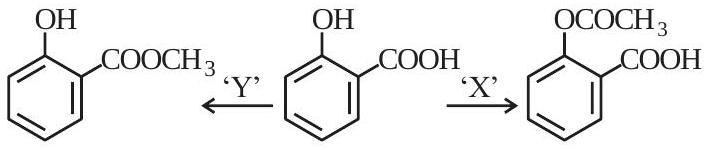
\includegraphics[max width=\textwidth, center]{2025_10_02_a54bf82dc4585184bb5fg-1(5)}\\
reagents ' X ' and ' Y ' respectively are :\\
(1) \(\left(\mathrm{CH}_{3} \mathrm{CO}\right)_{2} \mathrm{O} / \mathrm{H}^{+}\)and \(\mathrm{CH}_{3} \mathrm{OH} / \mathrm{H}^{+}, \Delta\)\\
(2) \(\left(\mathrm{CH}_{3} \mathrm{CO}\right)_{2} \mathrm{O} / \mathrm{H}^{+}\)and \(\left(\mathrm{CH}_{3} \mathrm{CO}\right)_{2} \mathrm{O} / \mathrm{H}^{+}\)\\
(3) \(\mathrm{CH}_{3} \mathrm{OH} / \mathrm{H}^{+}, \Delta\) and \(\mathrm{CH}_{3} \mathrm{OH} / \mathrm{H}^{+}, \Delta\)\\
(4) \(\mathrm{CH}_{3} \mathrm{OH} / \mathrm{H}^{+} \Delta\) and \(\left(\mathrm{CH}_{3} \mathrm{CO}\right)_{2} \mathrm{O} / \mathrm{H}^{+}\)
\end{enumerate}

Official Ans. by NTA (1)\\
Allen Ans. (1)

Sol.\\
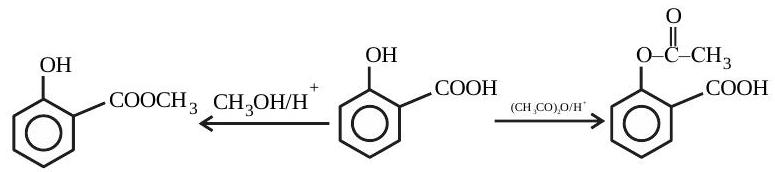
\includegraphics[max width=\textwidth, center]{2025_10_02_a54bf82dc4585184bb5fg-1}\\
32. The correct order of bond enthalpy \(\left(\mathrm{kJ} \mathrm{mol}^{-1}\right)\) is :\\
(1) \(\mathrm{Si}-\mathrm{Si}>\mathrm{C}-\mathrm{C}>\mathrm{Sn}-\mathrm{Sn}>\mathrm{Ge}-\mathrm{Ge}\)\\
(2) \(\mathrm{Si}-\mathrm{Si}>\mathrm{C}-\mathrm{C}>\mathrm{Ge}-\mathrm{Ge}>\mathrm{Sn}-\mathrm{Sn}\)\\
(3) \(\mathrm{C}-\mathrm{C}>\mathrm{Si}-\mathrm{Si}>\mathrm{Sn}-\mathrm{Sn}>\mathrm{Ge}-\mathrm{Ge}\)\\
(4) \(\mathrm{C}-\mathrm{C}>\mathrm{Si}-\mathrm{Si}>\mathrm{Ge}-\mathrm{Ge}>\mathrm{Sn}-\mathrm{Sn}\)

Official Ans. by NTA (4)\\
Allen Ans. (4)\\
Sol. (Bond enthalpy order\\
\(\mathbf{C}-\mathrm{C}>\mathrm{Si}-\mathrm{Si}>\mathrm{Ge}-\mathrm{Ge}>\mathrm{Sn}-\mathrm{Sn}\) )\\
33. All structures given below are of vitamin C. Most stable of them is :

(1)\\
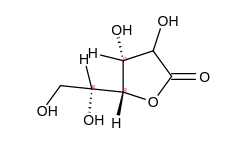
\includegraphics{smile-e9257e05ba6d1bc40b30b0f94db7b025474e320a}

(2)\\
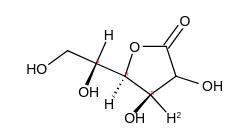
\includegraphics{smile-085a61e78305b71548050924c9b838180d91797c}

(3)\\
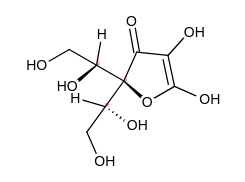
\includegraphics{smile-ffd8877558aeaa2c07f9011a6224f5f6e8b788d1}

(4)\\
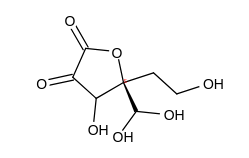
\includegraphics{smile-16a52fbb09d10e0fb8d19da0c54b9b50ee3a8ea0}

Official Ans. by NTA (1)\\
Allen Ans. (1)\\
Sol. H-bonding stabilised vitamin C\\
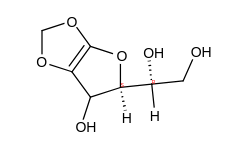
\includegraphics{smile-241821a1a2b3dc72f8b78b7bda8b0630f949793e}

\begin{figure}[h]
\begin{center}
\captionsetup{labelformat=empty}
\caption{(1)}
  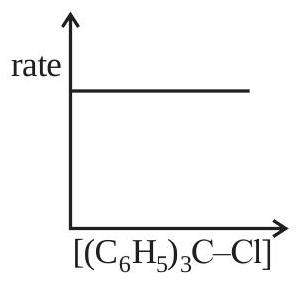
\includegraphics[width=\textwidth]{2025_10_02_a54bf82dc4585184bb5fg-1(3)}
\end{center}
\end{figure}

\begin{figure}[h]
\begin{center}
\captionsetup{labelformat=empty}
\caption{(3)}
  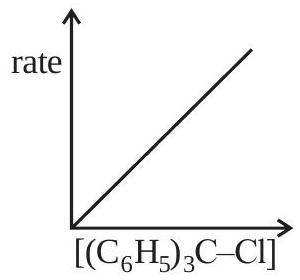
\includegraphics[width=\textwidth]{2025_10_02_a54bf82dc4585184bb5fg-1(7)}
\end{center}
\end{figure}

\begin{figure}[h]
\begin{center}
\captionsetup{labelformat=empty}
\caption{(2)}
  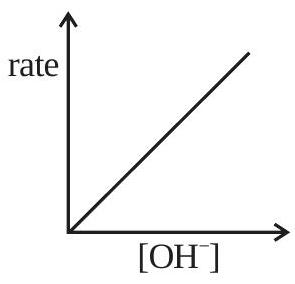
\includegraphics[width=\textwidth]{2025_10_02_a54bf82dc4585184bb5fg-1(4)}
\end{center}
\end{figure}

\begin{figure}[h]
\begin{center}
\captionsetup{labelformat=empty}
\caption{(4)}
  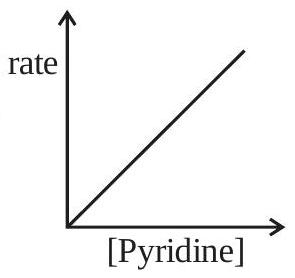
\includegraphics[width=\textwidth]{2025_10_02_a54bf82dc4585184bb5fg-1(1)}
\end{center}
\end{figure}

\section*{TEST PAPER WITH SOLUTION}
\begin{enumerate}
  \setcounter{enumi}{33}
  \item The graph which represents the following reaction is :\\
\(\left(\mathrm{C}_{6} \mathrm{H}_{5}\right)_{3} \mathrm{C}-\mathrm{Cl} \xrightarrow[\text { Pyridine }]{\mathrm{OH}^{-}}\left(\mathrm{C}_{6} \mathrm{H}_{5}\right)_{3} \mathrm{C}-\mathrm{OH}\)
\end{enumerate}

Official Ans. by NTA (3)\\
Allen Ans. (3)\\
Sol. (It is SN1 reaction so rate of reaction depends on the concentration of alkyl halide only.\\
35. ' X ' is :\\
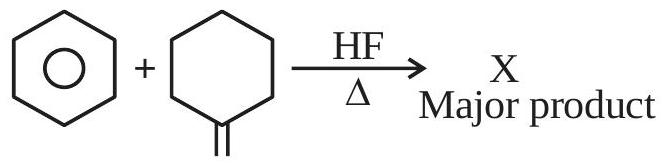
\includegraphics[max width=\textwidth, center]{2025_10_02_a54bf82dc4585184bb5fg-1(2)}

(1)\\
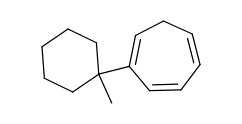
\includegraphics{smile-435b183677c4efdcfc56c64225a692e989160456}

(2)\\
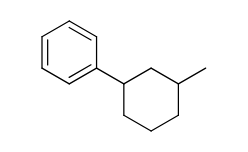
\includegraphics{smile-d7457d92db6bb63e8440253d18ad2e4b48b61956}

(3)\\
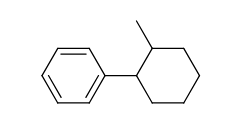
\includegraphics{smile-5eb068649fd86b4920bf17040d8ab04b2aec3960}

(4)\\
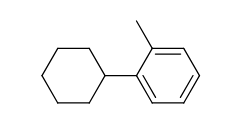
\includegraphics{smile-f47aa959dc8e7555b88409bb64f9a878d4203353}

Official Ans. by NTA (1)\\
Allen Ans. (1)\\
Sol.\\
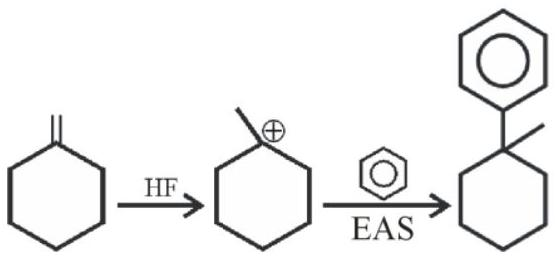
\includegraphics[max width=\textwidth, center]{2025_10_02_a54bf82dc4585184bb5fg-1(6)}\\
36. The complex cation which has two isomers is :\\
(1) \(\left[\mathrm{Co}\left(\mathrm{H}_{2} \mathrm{O}\right)_{6}\right]^{3+}\)\\
(2) \(\left[\mathrm{Co}\left(\mathrm{NH}_{3}\right)_{5} \mathrm{Cl}\right]^{2+}\)\\
(3) \(\left[\mathrm{Co}\left(\mathrm{NH}_{3}\right)_{5} \mathrm{NO}_{2}\right]^{2+}\)\\
(4) \(\left[\mathrm{Co}\left(\mathrm{NH}_{3}\right)_{5} \mathrm{Cl}\right]^{+}\)

Official Ans. by NTA (3)\\
Allen Ans. (3)\\
Sol. \(\left(\left[\mathrm{Co}\left(\mathrm{NH}_{3}\right)_{5} \mathrm{NO}_{2}\right]^{2+}\right.\)\\
Two linkage isomers possible\\
\(\mathrm{NO}_{2} \rightarrow\) Ambidentate ligand\\
37. Given below are two statements :

Statement I : Sulphanilic acid gives esterification test for carboxyl group.\\
Statement II : Sulphanilic acid gives red colour in Lassigne's test for extra element detection.\\
In the light of the above statements, choose the most appropriate answer from the options given below :\\
(1) Statement I is correct but Statement II is incorrect.\\
(2) Both Statement I and Statement II are incorrect.\\
(3) Both Statement I and Statement II are correct.\\
(4) Statement I is incorrect but Statement II is correct.\\
Official Ans. by NTA (4)\\
Allen Ans. (4)

Sol.\\
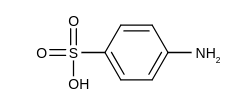
\includegraphics{smile-f2bb37ddf2fcb2b1519de2ad57d8daa8eb118fe4}

Does not show esterification test.\\
Presence of both sulphur and nitrogen give red colour in Lassigne's test.\\
38. Given below are two statements : one is labelled as Assertion (A) and the other is labelled as Reason (R).\\
Assertion (A) : Gypsum is used for making fireproof wall boards.\\
Reason (R) : Gypsum is unstable at high temperatures.\\
In the light of the above statements, choose the correct answer from the options given below :\\
(1) Both (A) and (R) are correct but (R) is not the correct explanation of (A).\\
(2) (A) is correct but (R) is not correct.\\
(3) (A) is not correct but (R) is correct.\\
(4) Both (A) and (R) are correct and (R) is the correct explanation of (A).\\
Official Ans. by NTA (1)\\
Allen Ans. (1)\\
Sol. (Gypsum is used for making fireproof wall boards.\\
39. Which element is not present in Nessler's reagent ?\\
(1) Mercury\\
(2) Potassium\\
(3) Iodine\\
(4) Oxygen

Official Ans. by NTA (4)\\
Allen Ans. (4)\\
Sol. (Nessler's Reagent \(\rightarrow \mathrm{K}_{2}\left[\mathrm{HgI}_{4}\right]\)\\
40. Given below are two statements : one is labelled as Assertion (A) and the other is labelled as Reason (R).

Assertion (A) : \(\alpha\)-halocarboxylic acid on reaction with dil. \(\mathrm{NH}_{3}\) gives good yield of \(\alpha\)-amino carboxylic acid whereas the yield of amines is very low when prepared from alkyl halides.

Reason (R) : Amino acids exist in zwitter ion form in aqueous medium.

In the light of the above statements, choose the correct answer from the options given below :\\
(1) Both (A) and (R) are correct and (R) is the correct explanation of (A).\\
(2) Both (A) and (R) are correct but (R) is not the correct explanation of (A).\\
(3) (A) is correct but (R) is not correct.\\
(4) (A) is not correct but (R) is correct.

Official Ans. by NTA (1)\\
Allen Ans. (2)\\
41. The industrial activity held least responsible for global warming is :\\
(1) manufacturing of cement\\
(2) steel manufacturing\\
(3) Electricity generation in thermal power plants.\\
(4) Industrial production of urea

Official Ans. by NTA (4)\\
Allen Ans. (4)\\
Sol. In urea production \(\mathrm{NH}_{3}\) and \(\mathrm{CO}_{2}\) consumed so least responsible for global warming.\\
42. The structures of major products \(\mathrm{A}, \mathrm{B}\) and C in the following reaction are sequence.\\
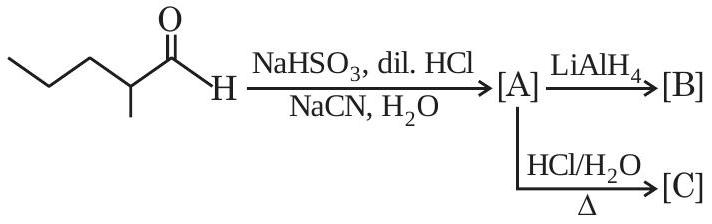
\includegraphics[max width=\textwidth, center]{2025_10_02_a54bf82dc4585184bb5fg-3}\\
(1)\\
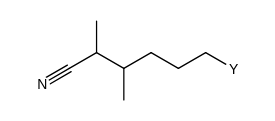
\includegraphics{smile-13ecc4c125ab70bb1de64b181b53e74c42b0cb0d}\\
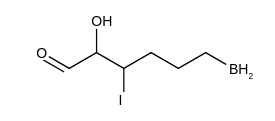
\includegraphics{smile-86e94a9e6e34c2b215e0c4a3d149670b217daf17}\\
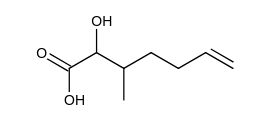
\includegraphics{smile-9e275ed13d42e2644c944580ae7a3d41c3cee138}\\
(2)\\
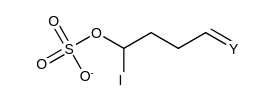
\includegraphics{smile-9291fbaeefa766594e122d44fef8ef70ced0d8cc}\\
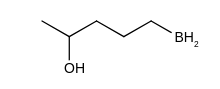
\includegraphics{smile-14dd4e4685ab70b96f6fffd8ca65d1789ed7df08}\\
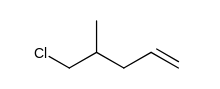
\includegraphics{smile-9a853e81853682edad0e14412603e6539fcf709c}\\
(3)\\
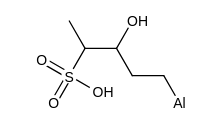
\includegraphics{smile-cb476d59bcc8da16a3bdd1d2a6859d76dc9d1937}\\
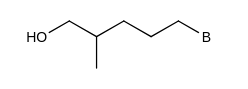
\includegraphics{smile-4cc67497d98ef15442dab8abff1abb6d61401f3c}\\
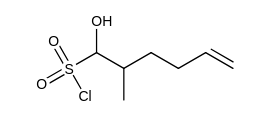
\includegraphics{smile-8a6421d2581512c4c8c4898d79c5d9262a92b5b9}\\
(4)\\
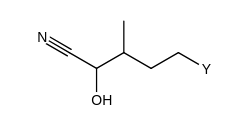
\includegraphics{smile-6cecab6ba6c51d23896f779aa7e4ff5a1443a33b}\\
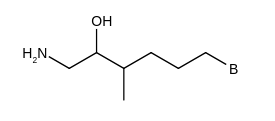
\includegraphics{smile-f3ac4c46d91342c877a1d3e0fa8a218360879b3e}\\
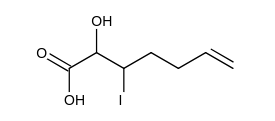
\includegraphics{smile-ae17fe8e360f820e334aea0ccf4ef6651bfae28c}

Official Ans. by NTA (4)\\
Allen Ans. (4)\\
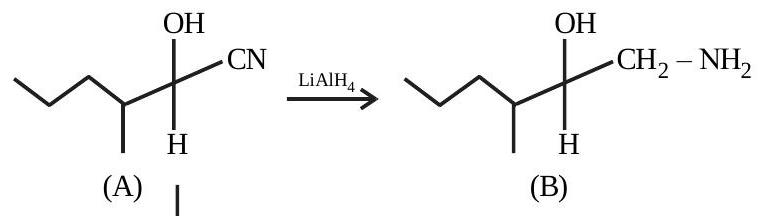
\includegraphics[max width=\textwidth, center]{2025_10_02_a54bf82dc4585184bb5fg-3(1)}

Sol.\\
43. Given below are two statements : one is labelled as Assertion (A) and the other is labelled as Reason (R).\\
Assertion (A) : \(\mathrm{Cu}^{2+}\) in water is more stable than \(\mathrm{Cu}^{+}\).\\
Reason (R) : Enthalpy of hydration for \(\mathrm{Cu}^{2+}\) is much less than that of \(\mathrm{Cu}^{+}\).

In the light of the above statements, choose the correct answer from the options given below :\\
(1) Both (A) and (R) are correct and (R) is the correct explanation of (A).\\
(2) (A) is correct but (R) is not correct.\\
(3) (1) is not correct but (R) is correct.\\
(4) Both (A) and (R) are correct but (R) is not the correct explanation of (A).\\
Official Ans. by NTA (1)\\
Allen Ans. (1)\\
Sol. \(\quad 2 \mathrm{Cu}^{+} \rightarrow \mathrm{Cu}^{2+}+\mathrm{Cu}\)\\
The stability of \(\mathrm{Cu}^{2+}(\mathrm{aq})\) rather than \(\mathrm{Cu}^{+}(\mathrm{aq})\), is due to the much more negative \(\Delta_{\text {hyd }} \mathrm{H}\) of \(\mathrm{Cu}^{2+}(\mathrm{aq})\) than \(\mathrm{Cu}^{+}(\mathrm{aq})\), which more than compensates for the second ionisation enthalpy of Cu .\\
44. The starting material for convenient preparation of deuterated hydrogen peroxide ( \(\mathrm{D}_{2} \mathrm{O}_{2}\) ) in laboratory is:\\
(1) \(\mathrm{K}_{2} \mathrm{~S}_{2} \mathrm{O}_{8}\)\\
(2) 2-ethylanthraquinol\\
(3) \(\mathrm{BaO}_{2}\)\\
(4) BaO

Official Ans. by NTA (1)\\
Allen Ans. (1)\\
Sol. \(\quad\left(\mathrm{K}_{2} \mathrm{~S}_{2} \mathrm{O}_{8}(\mathrm{~s})+2 \mathrm{D}_{2} \mathrm{O}(\mathrm{l}) \rightarrow 2 \mathrm{KDSO}_{4}(\mathrm{aq})+.\mathrm{D}_{2} \mathrm{O}_{2}\right.\)\\
45. In figure, a straight line is given for Freundrich Adsorption \((y=3 x+2.505)\). The value of \(\frac{1}{n}\) and \(\log \mathrm{K}\) are respectively.\\
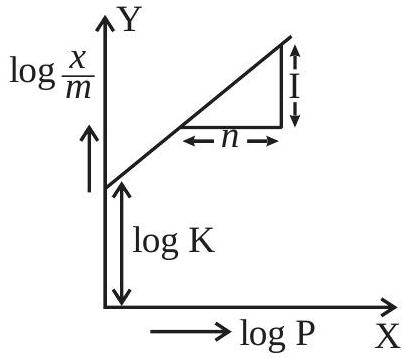
\includegraphics[max width=\textwidth, center]{2025_10_02_a54bf82dc4585184bb5fg-3(2)}\\
(1) 0.3 and \(\log 2.505\)\\
(2) 0.3 and 0.7033\\
(3) 3 and 2.505\\
(4) 3 and 0.7033

Official Ans. by NTA (3)\\
Allen Ans. (3)

Sol. \(\frac{X}{m}=K p^{1 / n}\)\\
\(\log \frac{\mathrm{x}}{\mathrm{m}}=\log \mathrm{k}+\frac{1}{\mathrm{n}} \log \mathrm{P}\)\\
\(Y=3 x+2.505, \frac{1}{n}=3, \log K=2.505\) )\\
46. Given below are two statements : one is labelled as

Assertion (A) and the other is labelled as Reason (R).

Assertion (A) : An aqueous solution of KOH when for volumetric analysis, its concentration should be checked before the use.

Reason (R) : On aging, KOH solution absorbs atmospheric \(\mathrm{CO}_{2}\).

In the light of the above statements, choose the correct answer from the options given below.\\
(1) (A) is not correct but (R) is correct\\
(2) Both (A) and (R) are correct but (R) is not the correct explanation of (A)\\
(3) Both (A) and (R) are correct and (R) is the correct explanation of (A)\\
(4) (A) is correct but (R) is not correct

Official Ans. by NTA (3)\\
Allen Ans. (3)\\
Sol. KOH absorb \(\mathrm{CO}_{2}\)\\
So its concentration should be checked.\\
47. Which one of the following sets of ions represents a collection of isoelectronic species?\\
(Given : Atomic Number : \(\mathrm{F}: 9, \mathrm{Cl}: 17, \mathrm{Na}=11\),\\
\(\mathrm{Mg}=12, \mathrm{Al}=13, \mathrm{~K}=19, \mathrm{Ca}=20, \mathrm{Sc}=21\) )\\
(1) \(\left(\mathrm{Li}^{+}, \mathrm{Na}^{+}, \mathrm{Mg}^{2+}, \mathrm{Ca}^{2+}\right.\)\\
(2) \(\left(\mathrm{Ba}^{2+}, \mathrm{Sr}^{2+}, \mathrm{K}+, \mathrm{Ca}^{2+}\right.\)\\
(3) \(\left(\mathrm{N}^{3-}, \mathrm{O}^{2-}, \mathrm{F}^{-}, \mathrm{S}^{2-}\right.\)\\
(4) \(\left(\mathrm{K}^{+}, \mathrm{Cl}^{-}, \mathrm{Ca}^{2+}, \mathrm{Sc}^{3+}\right.\)

Official Ans. by NTA (4)\\
Allen Ans. (4)\\
Sol. \(\quad \begin{array}{cccc}\mathrm{K}^{+} & \mathrm{Cl}^{1} & \mathrm{Ca}^{2+} & \mathrm{Sc}^{3+} \\ & 18 & 18 & 18\end{array}\)\\
48. The effect of addition of helium gas to the following reaction in equilibrium state, is :\\
\(\mathrm{PCI}_{5}(\mathrm{~g}) \rightleftharpoons \mathrm{PCl}_{3}(\mathrm{~g})+\mathrm{Cl}_{2}(\mathrm{~g})\)\\
(1) the equilibrium will shift in the forward direction and more of \(\mathrm{Cl}_{2}\) and \(\mathrm{PCl}_{3}\) gases will be produced.\\
(2) the equilibrium will go backward due to suppression of dissociation of \(\mathrm{PCl}_{5}\).\\
(3) helium will deactivate \(\mathrm{PCl}_{5}\) and reaction will stop.\\
(4) addition of helium will not affect the equilibrium.

Official Ans. by NTA (1)\\
Allen Ans. (A \& D)\\
Sol. \(\mathrm{PCI}_{5}(\mathrm{~g}) \rightleftharpoons \mathrm{PCl}_{3}(\mathrm{~g})+\mathrm{Cl}_{2}(\mathrm{~g})\)\\
(Case 1 : At constant P - volume will increase so reaction will shift in forward direction then answer will be A

Case 2 : At constant volume no change in active mass so reaction will not shift in any direction then answer will be D .\\
49. For electron gain enthalpies of the elements denoted as \(\Delta_{\mathrm{eg}} \mathrm{H}\), the incorrect option is :\\
(1) \(\Delta_{\mathrm{eg}} \mathrm{H}(\mathrm{Cl})<\Delta_{\mathrm{eg}} \mathrm{H}(\mathrm{F})\)\\
(2) \(\Delta_{\mathrm{eg}} \mathrm{H}(\mathrm{Se})<\Delta_{\mathrm{eg}} \mathrm{H}(\mathrm{S})\)\\
(3) \(\Delta_{\mathrm{eg}} \mathrm{H}(\mathrm{I})<\Delta_{\mathrm{eg}} \mathrm{H}(\mathrm{At})\)\\
(4) \(\Delta_{\mathrm{eg}} \mathrm{H}(\mathrm{Te})<\Delta_{\mathrm{eg}} \mathrm{H}(\mathrm{Po})\)

Official Ans. by NTA (2)\\
Allen Ans. (2)\\
Sol. (1) \(\Delta_{\mathrm{eg}} \mathrm{H}(\mathrm{Cl})<\Delta_{\mathrm{eg}} \mathrm{H}(\mathrm{F})\)\\
(-345) (-328) Correct\\
(2) \(\Delta_{\mathrm{eg}} \mathrm{H}(\mathrm{Se})<\Delta_{\mathrm{eg}} \mathrm{H}(\mathrm{S})\)\\
(-195) (-200) Incorrect\\
(3) \(\Delta_{\mathrm{eg}} \mathrm{H}(\mathrm{I})<\Delta_{\mathrm{eg}} \mathrm{H}(\mathrm{At})\)\\
(-295) (-270) Correct\\
(4) \(\Delta_{\mathrm{eg}} \mathrm{H}(\mathrm{Te})<\Delta_{\mathrm{eg}} \mathrm{H}(\mathrm{Po})\)\\
(-190) (-183) Correct\\
50. \(\mathrm{O}-\mathrm{O}\) bond length in \(\mathrm{H}_{2} \mathrm{O}_{2}\) is \(\underline{\mathrm{X}}\) than the \(\mathrm{O}-\mathrm{O}\) bond length in \(\mathrm{F}_{2} \mathrm{O}_{2}\). The \(\mathrm{O}-\mathrm{H}\) bond length in \(\mathrm{H}_{2} \mathrm{O}_{2}\) is \(\underline{\mathrm{Y}}\) than that of the \(\mathrm{O}-\mathrm{F}\) bond in \(\mathrm{F}_{2} \mathrm{O}_{2}\).\\
Choose the correct option for \(\underline{X}\) and \(\underline{Y}\) from the given below.

\begin{center}
\begin{tabular}{ll}
(1) \(X-\) shorter, & \(Y-\) shorter \\
(2) \(X-\) shorter, & \(Y-\) longer \\
(3) \(X-\) longer, & \(Y-\) longer \\
(4) \(X-\) longer, & \(Y-\) shorter \\
\end{tabular}
\end{center}

Official Ans. by NTA (4)\\
Allen Ans. (4)\\
Sol. According to bent rule more electronegative atom occupy less s-characters so bond length increases. \(\mathrm{O}-\mathrm{H}\) bond will be short than \(\mathrm{O}-\mathrm{F}\) bond due to small size of H than F .

\section*{SECTION-B}
\begin{enumerate}
  \setcounter{enumi}{50}
  \item 0.3 g of ethane undergoes combustion at \(27^{\circ} \mathrm{C}\) in a bomb calorimeter. The temperature of calorimeter system (including the water) is found to rise by \(0.5^{\circ} \mathrm{C}\). The heat evolved during combustion of ethane at constant pressure is \(\_\_\_\_\) \(\mathrm{kJ} \mathrm{mol}^{-1}\).\\
(Nearest integer)\\[0pt]
[Given : The heat capacity of the calorimeter system is \(20 \mathrm{~kJ} \mathrm{~K}^{-1}, \mathrm{R}=8.3 \mathrm{JK}^{-1} \mathrm{~mol}^{-1}\).
\end{enumerate}

Assume ideal gas behaviour.\\
Atomic mass of C and H are 12 and \(1 \mathrm{~g} \mathrm{~mol}^{-1}\) respectively]

Official Ans. by NTA (1006)\\
Allen Ans. (1006)\\
Sol. (Bomb calorimeter \(\rightarrow\) const volume\\
Heat released\\
By combustion of 1 mole\\
\(\mathrm{C}_{2} \mathrm{H}_{6}(\Delta \mathrm{U})=-\frac{20 \times 0.5}{0.3} \times 30=-1000 \mathrm{~kJ}\)\\
\(\mathrm{C}_{2} \mathrm{H}_{6}(\mathrm{~g})+7 / 2 \mathrm{O}_{2}(\mathrm{~g}) \rightarrow 2 \mathrm{CO}_{2}(\mathrm{~g})+3 \mathrm{H}_{2} \mathrm{O}(l)\)\\
\(\Delta \mathrm{ng}=2-(2+7 / 2)=-(7 / 2)\)\\
\(\Delta \mathrm{H}=\Delta \mathrm{U}+\Delta \mathrm{nRT}\)\\
\(=-1000-7 / 2 \times 8.3 \times 300 \mathrm{~kJ}\)\\
\(=-1000-6.225\)\\
\(=-1006 \mathrm{~kJ}\)\\
So heat released \(=1006 \mathrm{~kJ} \mathrm{~mol}^{-1}\)\\
52. Among following compounds, the number of those present in copper matte is \(\_\_\_\_\) .\\
A. \(\mathrm{CuCO}_{3}\)\\
B. \(\mathrm{Cu}_{2} \mathrm{~S}\)\\
C. \(\mathrm{Cu}_{2} \mathrm{O}\)\\
D. FeO

Official Ans. by NTA (3)\\
Allen Ans. (1)\\
Sol. FeS and \(\mathrm{Cu}_{2} \mathrm{~S}\), present in copper matte.\\
53. Among the following, the number of tranquilizer/s is/are \(\_\_\_\_\) .\\
A. Chloroliazepoxide\\
B. Veronal\\
C. Valium\\
D. Salvarsan

Official Ans. by NTA (3)\\
Allen Ans. (3)\\
Sol. (chlorodiazepoxide, Veronal, Valium is tranquilizer where as salvarsan is antibiotic.\\
54. \(\mathrm{A} \rightarrow \mathrm{B}\)

The above reaction is of zero order. Half life of this reaction is 50 min . The time taken for the concentration of A to reduce to one-fourth of its initial value is \(\_\_\_\_\) min.\\
(Nearest integer)\\
Official Ans. by NTA (75)\\
Allen Ans. (75)\\
Sol. Assume reaction starts with 1 mole A\\
( \(\mathrm{t}_{1 / 2}=\frac{\mathrm{a}}{2 \mathrm{k}}, \mathrm{K}=\frac{1}{2 \times 50}\)\\
For 75\% completion\\
\(\mathrm{a}-\frac{\mathrm{a}}{4}=\mathrm{kt}\)\\
\(\mathrm{t}=\frac{3}{4} \frac{\mathrm{a}}{\mathrm{k}}=\frac{3}{4} \times \frac{100}{\mathrm{a}}=75\)\\
55. \(20 \%\) of acetic acid is dissociated when its 5 g is added to 500 mL of water. The depression in freezing point of such water is \(\_\_\_\_\) \(\times 10^{-3}{ }^{\circ} \mathrm{C}\). Atomic mass of \(\mathrm{C}, \mathrm{H}\) and O are 12, 1 and 16 a.m.u. respectively.\\[0pt]
[Given : Molal depression constant and density of water are \(1.86 \mathrm{~K} \mathrm{~kg} \mathrm{~mol}^{-1}\) and \(1 \mathrm{~g} \mathrm{~cm} \mathrm{~cm}^{-3}\) respectively.

Official Ans. by NTA (372)\\
Allen Ans. (372)\\
Sol. \(\quad i=1+(n-1) \alpha\)\\
\((\mathrm{i}=1+0.2(2-1)=1.2\)\\
\(\Delta \mathrm{T}_{\mathrm{f}}=\mathrm{i} \mathrm{K}_{\mathrm{f}} \mathrm{m}\)\\
\(\Delta \mathrm{T}_{\mathrm{f}}=1.2 \times 1.86 \times \frac{5 \times 1000}{60 \times 500}\)\\
\(\Delta \mathrm{t}_{\mathrm{f}}=3.72\)\\
\(\Delta \mathrm{T}_{\mathrm{f}}=372 \times 10^{-2}\)\\
56. The molality of a \(10 \%(\mathrm{v} / \mathrm{v})\) solution of di-bromine solution in \(\mathrm{CCl}_{4}\) (carbon tetrachloride) is ' \(x\) '. \(x=\)\\
\(\_\_\_\_\) \(\times 10^{-2} \mathrm{M}\). (Nearest integer)\\[0pt]
[Given : molar mass of \(\mathrm{Br}_{2}=160 \mathrm{~g} \mathrm{~mol}^{-1}\)\\
atomic mass of \(\mathrm{C}=12 \mathrm{~g} \mathrm{~mol}^{-1}\)\\
atomic mass of \(\mathrm{Cl}=35.5 \mathrm{~g} \mathrm{~mol}^{-1}\)\\
density of dibromine \(=3.2 \mathrm{~g} \mathrm{~cm}^{-3}\)\\
density of \(\mathrm{CCl}_{4}=1.6 \mathrm{~g} \mathrm{~cm}^{-3}\) ]\\
Official Ans. by NTA (139)\\
Allen Ans. (139)\\
Sol. ( 10 ml solute in 90 ml solvent\\
mass of solute \(=10 \times 3.2=32 \mathrm{~g}\)\\
mass of solvent \(=90 \times 1.6 \mathrm{~g}\)\\
\(\mathrm{m}=\frac{32 \times 1000}{160 \times 90 \times 1.6}=1.388\)\\
\(\mathrm{m}=138.8 \times 10^{-2}=139\)\\
57. \(1 \times 10^{-5} \mathrm{M} \mathrm{AgNO}_{3}\) is added to 1 L of saturated solution of AgBr . The conductivity of this solution at 298 K is \(\_\_\_\_\) \(\times 10^{-8} \mathrm{~S} \mathrm{~m}^{-1}\).\\[0pt]
[Given : \(\mathrm{K}_{\text {sp }}(\mathrm{AgBr})=4.9 \times 10^{-13}\) at 298 K\\
\(\lambda_{\mathrm{Ag}^{+}}^{0}=6 \times 10^{-3} \mathrm{Sm}^{2} \mathrm{~mol}^{-1}\)\\
\(\lambda_{\mathrm{Br}^{-}}^{0}=8 \times 10^{-3} \mathrm{Sm}^{2} \mathrm{~mol}^{-1}\)\\
\(\left.\lambda_{\mathrm{NO}_{3}^{-}}^{0}=7 \times 10^{-3} \mathrm{Sm}^{2} \mathrm{~mol}^{-1}\right]\)

Official Ans. by NTA (14)\\
Allen Ans. (Bonus)\\
Sol. \(\left[\mathrm{Ag}^{+}\right]=10^{-5}\)\\
\(\left[\mathrm{NO}_{3}^{-}\right]=10^{-5}\)\\
\(\left[\mathrm{Br}^{-}\right]=\frac{\mathrm{Ksp}}{\left[\mathrm{Ag}^{+}\right]}=4.9 \times 10^{-8}\)\\
\(\Lambda_{\mathrm{m}}=\frac{\mathrm{k}}{1000 \times \mathrm{M}}\)

For \(\mathrm{Ag}^{+}\)\\
\(6 \times 10^{-3}=\frac{\mathrm{K}_{\mathrm{Ag}^{+}}}{1000 \times 10^{-5}}\)\\
\(\mathrm{K}_{\mathrm{Ag}+}=6 \times 10^{-5}\)\\
\(\Rightarrow 6000 \times 10^{-8}\)\\
for \(\mathrm{Br}^{-}\)\\
\(8 \times 10^{-3}=\frac{\mathrm{K}_{\mathrm{Br}^{-}}}{1000 \times 4.9 \times 10^{-8}}\)\\
\(\mathrm{K}_{\mathrm{Br}-}=39.2 \times 10^{-8}\)\\
for \(\mathrm{NO}_{3}^{-}\)\\
\(7 \times 10^{-3}=\frac{\mathrm{K}_{\mathrm{NO}_{3}^{-}}}{1000 \times 10^{-5}}\)\\
\(\mathrm{K}_{\mathrm{NO}_{3}^{-}}=7 \times 10^{-5}\)

\[
=7000 \times 10^{-8}
\]

Conductivity of solution\\
\(\Rightarrow(6000+7000+39.2) \times 10^{-8}\)\\
\(\Rightarrow 13039.2 \times 10^{-8} \mathrm{~S} \mathrm{~m}^{-1}\)\\
58. Testosterone, which is a steroidal hormone, has the following structure.\\
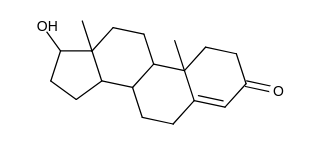
\includegraphics{smile-d9077d3b1d9617d063086722df23629eb1021228}

The total number of asymmetric carbon atom/s in testosterone is \(\_\_\_\_\)\\
Official Ans. by NTA (6)\\
Allen Ans. (6)

Sol.\\
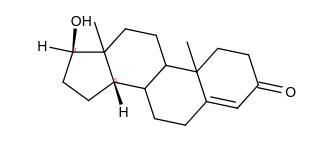
\includegraphics{smile-37987e303bafab6946418ffe3b8944b36368f49e}\\
59. The spin only magnetic moment of \(\left[\mathrm{Mn}\left(\mathrm{H}_{2} \mathrm{O}\right)_{6}\right]^{2+}\) complexes is \(\_\_\_\_\) B.M. (Nearest integer)\\
(Given : Atomic no. of Mn is 25 )

\section*{Official Ans. by NTA (6)}
Allen Ans. (6)\\
Sol. \(\left(\left[\mathrm{Mn}\left(\mathrm{H}_{2} \mathrm{O}\right)_{6}\right]^{2+}\right.\)\\
\(\mathrm{Mn}^{2+}=3 \mathrm{~d}^{5}\)\\
\(\mu=\sqrt{5(5+2)}=5.91 \mathrm{BM}\)\\
60. A metal M crystallizes into two lattices :- face centred cubic (fcc) and body centred cubic (bcc) with unit cell edge length of 2.0 and \(2.5 \AA\) respectively. The ratio of densities of lattices fcc to bcc for the metal M is \(\_\_\_\_\) .\\
(Nearest integer)

\section*{Official Ans. by NTA (4)}
Allen Ans. (4)\\
Sol. \(\mathrm{d}=\frac{\mathrm{Z} \times \mathrm{M}}{\mathrm{N}_{\mathrm{A}} \mathrm{a}^{3}}\)\\
\(\frac{d_{F C C}}{d_{B C C}}=\frac{\frac{4 \times M_{w}}{N_{A} \times(2)^{3}}}{\frac{2 \times M_{w}}{N_{A} \times(2.5)^{3}}}=3.90\)


\end{document}